% !TEX root = ../../book.tex

\chapter{Execution Fundamentals}

\section{A Brief History of Stock Trading}
Stoll (2006)~\cite{hstoll} in an instructive essay traces the evolution of trading that started under a tree in 1792 with 24 brokers. This has become later on the New York Stock Exchange (NYSE). Modern electronic technology has changed how trading is done. Now all transactions are carried out though a computer system with little human intervention (see the snapshots of NYSE over two different decades).
	\begin{figure}[!ht]
   	\centering
   	\includegraphics[width=0.9\textwidth]{chapters/chapter_trading_fund/figures/pit_trading.png} 
   	\caption{Treasury bind pit 1989. \label{fig:pittrade}}
	\end{figure}
	\begin{figure}[!ht]
	   \centering
	   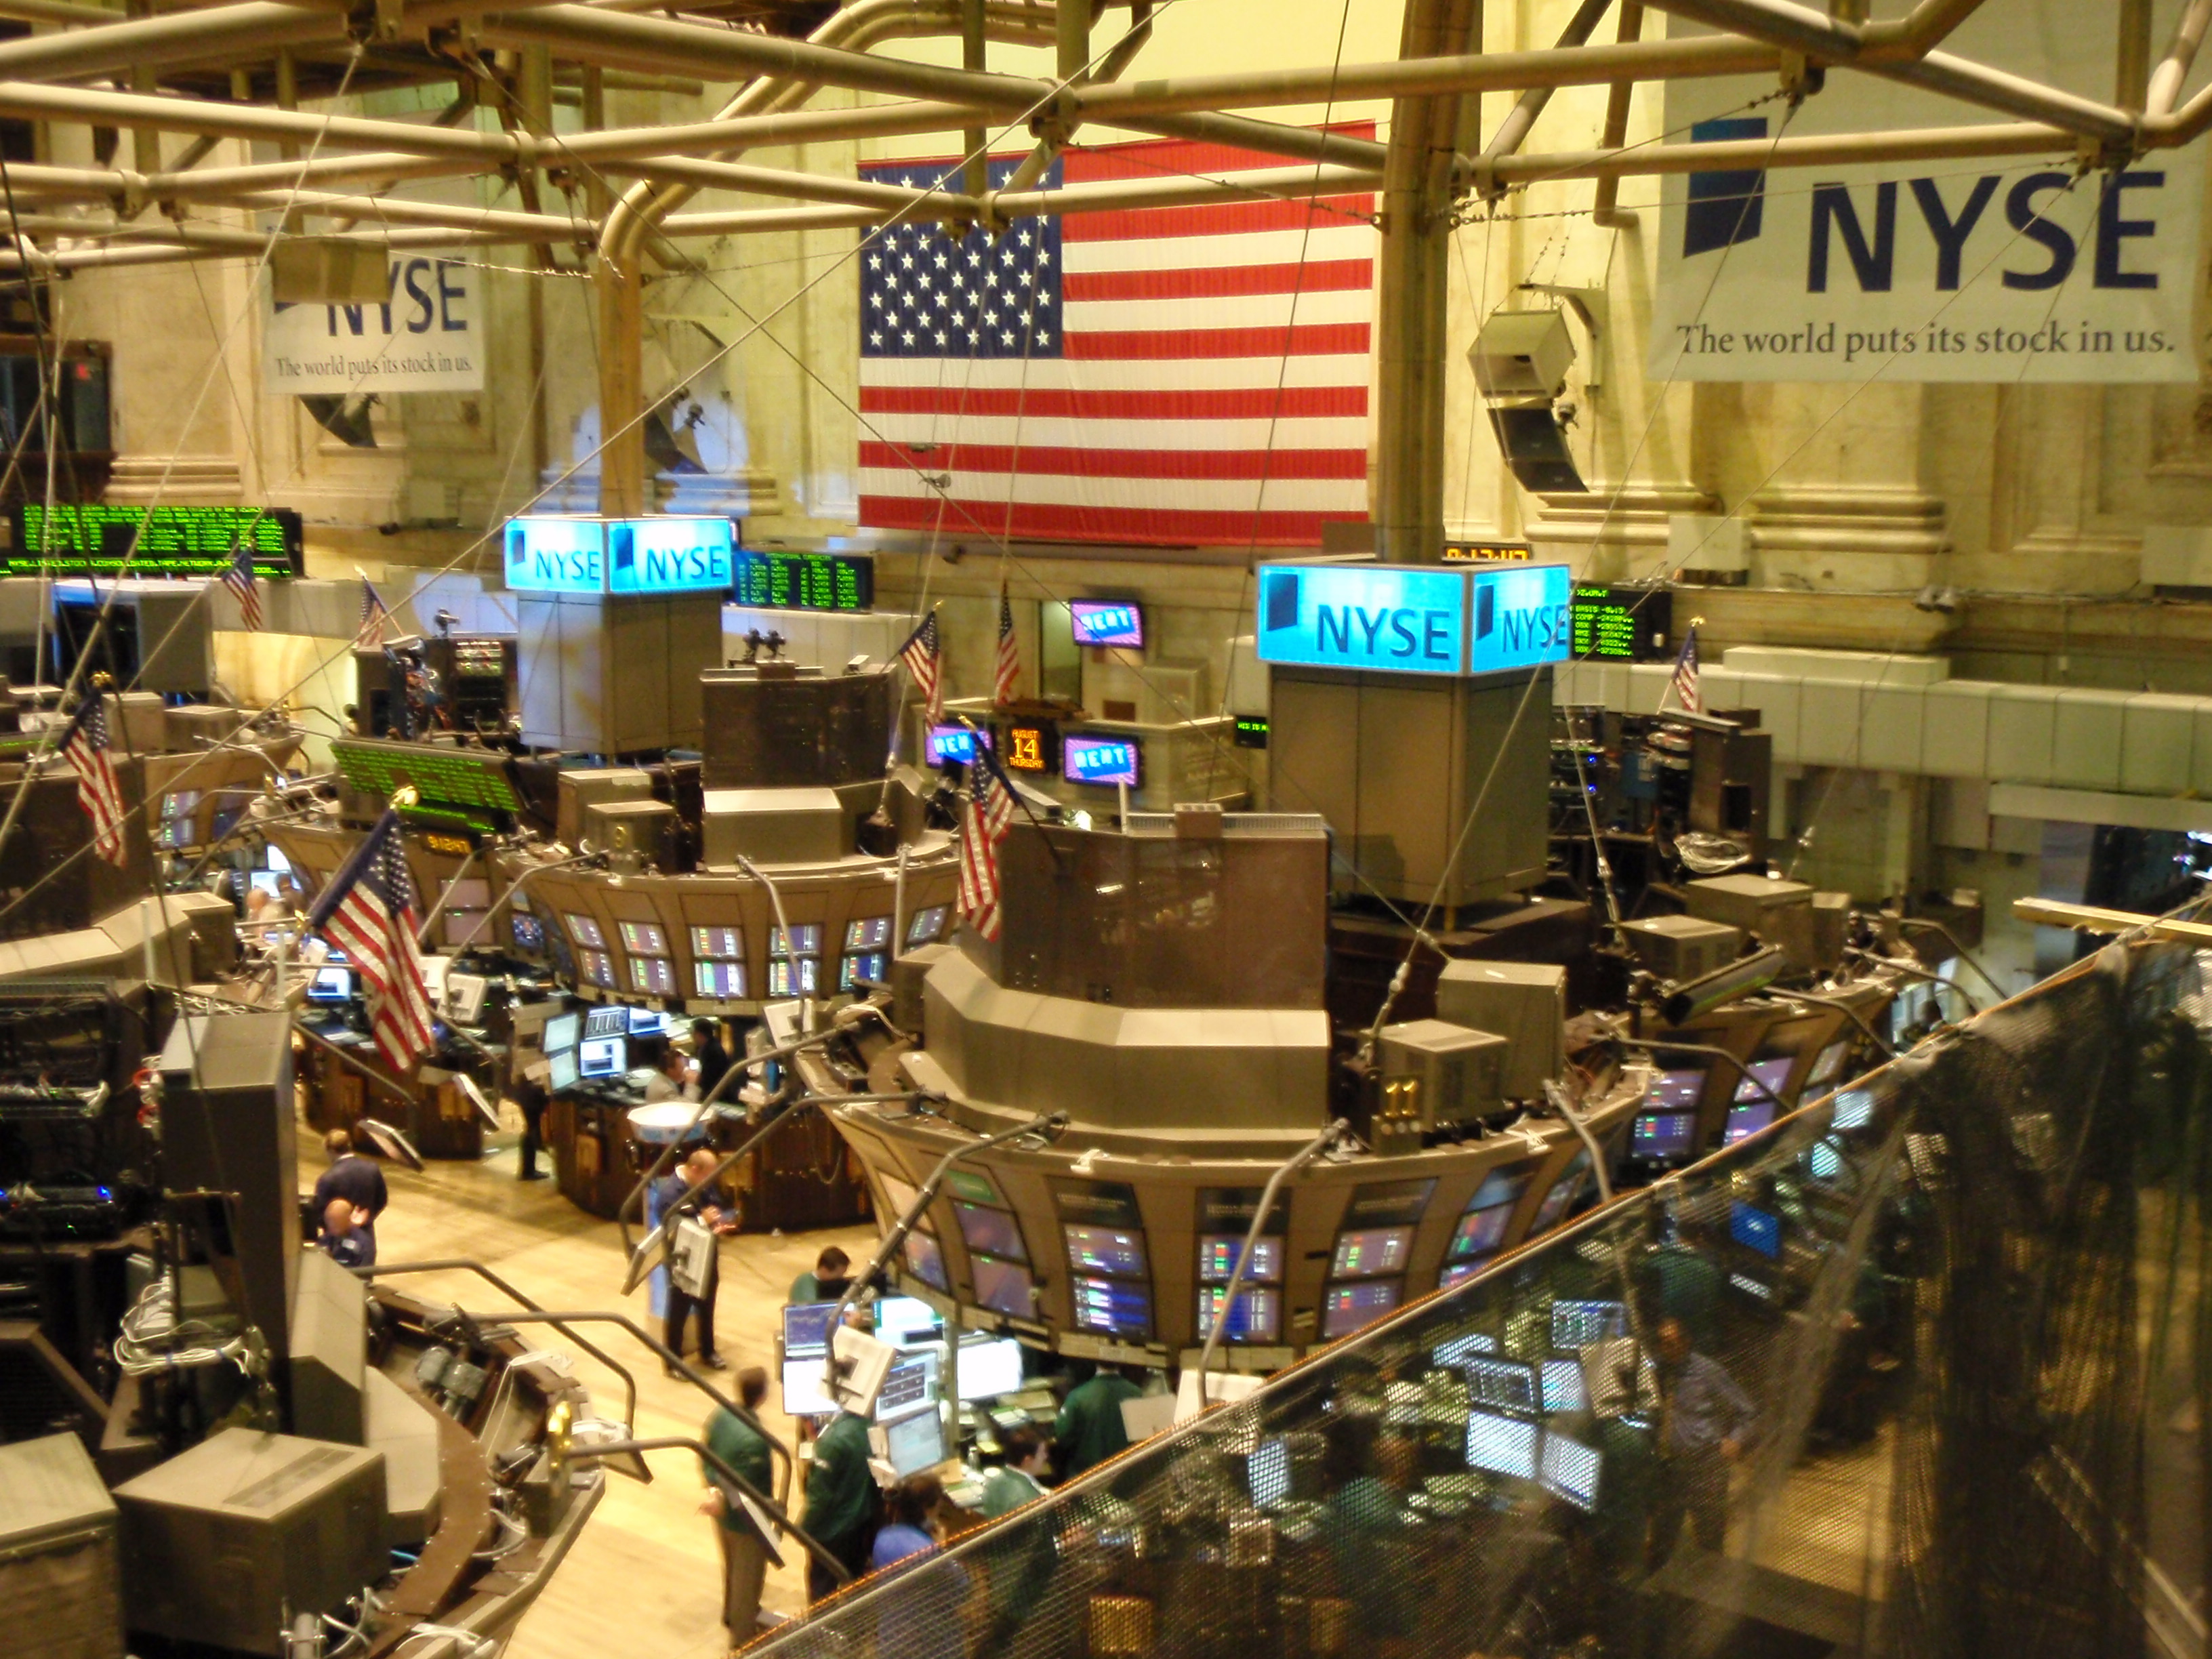
\includegraphics[width=0.9\textwidth]{chapters/chapter_trading_fund/figures/electronic_trading.png} 
	   \caption{The NYSE trading floor in August 2008. \label{fig:electrade}}
	\end{figure}
This has also changed how stock market trading is done. The Electronic Communication Networks (ECN) automate the trading process but the fundamental functions of trading are not changed except for the instant dissemination of the demand and supply information to all investors. The identity of traders is kept anonymous. Executions are done fast and very complex orders can now be submitted to the market. The trading costs---both direct such as commissions, brokerage fees, etc. and indirect cost due to price-impact---are expected to be lower. Over the period of two decades (1980--2000), the commissions have have gone down from 1.2\% to 0.2\%. But with higher turnover and thus with increased volume, the total commissions have increased four-fold. The reduction in bid-ask spread although may be primarily due to tick size is accelerated under electronic trading. 


It must be observed that electronic trading does not necessarily imply automated trading. But it has certainly led to more automated trading due to easy execution of the algorithms. Although there is a concern that the traders can game the prices, but computer audit trails can be used to monitor unlawful behaviors. The debate over whether electronification of trading will lead to more consolidation or fragmentation has favored the latter. The apprehension over the possibility of inefficient price formation due to fragmentation is empirically shown not to hold. The order protection rule (SEC 2005) that dictates that an order submitted to any market should get the best of prices in all markets. 


Thus large number of equity and derivative markets are now organized as electronic limit order books. The Electronic Communications Networks (ECNs) in the United States, Hong Kong and Toronto Stock Exchanges are examples of equity markets. Chicago Mercantile Exchange's (CME) Globex platform, Euronext Liffe's centralized limit order book are example of derivative markets. Open limit order books have become popular due to the greater transparency of the market when compared with dealer market settings, that rely upon the information on the dealers' best quotes. The limit order book provides its users to view the depth of the book at various price level away from the best quotes. In dealer market prices for trades beyond the quoted size must be obtained through negotiation with market maker. 


There has been a great deal of interest in studying the information content of an open limit order book and if it helps investors in tracking short-term price predictions. Assuming that the market consists of informed and noise traders, and the informed traders actively submit market orders, Glosten (1994)~\cite{glosten94} and Seppi (1997)~\cite{seppi97} argue that the order book does not contain any information beyond the best bid and best offer. But other studies such as Harris and Panchapagesan (2005)~\cite{harrispan} argue that the order book is informative and specialists better use the book information to their advantage than the traders who routinely place limit orders. In this chapter we discuss the feature of limit order book and various levels of information that have been made available to the investors; the focus is on developing models for studying the dynamics on the book and how the models could be used for high frequency trading. 


An excellent survey paper by Parlour and Seppi (2008)~\cite{parseppi} reviews the issues related to limit order markets. A limit order for any asset `$j$' is an  ex ante pre-commitment $(t,x,p)$ made at time `$t$' to trade `$x$' units at a pre-specified limit price, `$p$'. The order remains valid until it is filled or cancelled. With multiple exchanges, the interactions are quite complex; the dynamic nature of state of the order book and the choice of actions in anticipation of the future states make the limit order placement decisions, $(t,x,p)$ challenging. The key issues in the study of LOB are nicely summarized in Parlour and Seppi (2008)~\cite{parseppi}. They relate to, Price Formulation (How limit order markets differ from dynamic dealer markets?), Liquidity (Implication of the quotes posted at various depths in LOB), Dynamics (Dependencies of Various Trading Decisions), Information Aggregation (How forward-looking is the activity in LOB about future order flow in aggregate?) and Inter-Market Competition (How effective are limit order markets to induce competition and how they handle non-market frictions?). How multiple exchanges can sustain competitive pressure to attract postings to their venues? How do limit order markets help reduce market frictions? These issues are addressed in this chapter but our focus is always on how the information flow through LOB dynamics helps trading decisions. The tools we review here in this chapter can be useful to that end. 


\section{Market Structure and Trading Venues: A Review}
\section{The Mechanics of Trading: The Limit Order Book}

In automated continuous double auction trading system that have have become prevalent in the financial markets, buyers and sellers submit limit orders electronically; orders are then matched and executed as per time and price priorities. The unmatched orders are stored in the limit order book (LOB). The market orders are orders seeking the best available price and they are execute immediately. Thus, one way or other all executed orders can be taken as market orders.


The state of the order book changes quite rapidly due to high frequency program trading. There are six types of events, three on either side that can alter the state of the order book:
	\begin{itemize}
	\item Limit order submission: A limit order is added to the queue at the specified price level.
	\item Limit order cancellation: An outstanding limit order is expired or cancelled and therefore is removed from the LOB.
	\item Market order submission: Outstanding limit order at the best price are executed against the market order and thus removed from the book.
	\end{itemize}


Orders on the buy side are called ``bids'' while those on the sell side are called ``asks.'' The above events illustrated in the following diagrams.
	\begin{figure}[!ht]
	   \centering
	   \includegraphics[width=0.9\textwidth]{chapters/chapter_trading_fund/figures/limitbk1.png} 
	   \caption{Limit Order Book---Limit Bid. \label{fig:limbk1}}
	\end{figure}
	\begin{figure}[!ht]
	   \centering
	   \includegraphics[width=0.9\textwidth]{chapters/chapter_trading_fund/figures/limitbk2.png} 
	   \caption{Limit Order Book---Market Bid. \label{fig:limbk2}}
	\end{figure}
When a market order is submitted, it decreases the number of outstanding orders at the opposite best price. For example, if a market bid order arrives, it will decrease the number of outstanding asks at the best price.
	\begin{figure}[!ht]
	   \centering
	   \includegraphics[width=0.9\textwidth]{chapters/chapter_trading_fund/figures/limitbk3.png} 
	   \caption{Limit Order Book---Ask Cancellation. \label{fig:limbk3}}
	\end{figure}
All unexecuted limit orders can be cancelled. When a cancellation occurs, it will decrease the number of outstanding orders at the specified price level. 


The limit orders constitute a very significant percentage (70\%) of stock market trading activity. The main advantage of a limit order is that there is no price risk, that is when the order is executed the limit price is attained. But the execution is not guaranteed and the time to get an order executed depends on various market factors. The trade off between the limit order and the market order depends on the investors need for liquidity and the probability of execution of a limit order. The execution of limit orders does affect how the quotes are posted and are updated. A market order will be filled at or close to National Best Bid and Offer (NBBO). If the size of the order exceeds the number of shares available, it is usually split and is executed at different prices until the order is filled. The market orders are usually restricted to be filled within a day and order placed after the markets close are entered the next day at 9:30~am EST. Other types include stop-limit orders and trailing stop orders. The former type is typically used to trade a security at a specified limit price once it is traded through a specified stop price. If the stock declines in value and traders below or at the stop price, the order will become a limit order rather than a market order. The trailing stop order is in which the specified price will trail by a certain percentage from the best bid or best ask. These rules are handled in the brokers IT technology. In addition to time and duration specifications, other conditions that can be added are: fill or kill (the order gets filled in its entirety or not filled at all) or minimum quantity (if the specified minimum is not available, the order does not get executed).  

\subsection{How Double Auction Markets Work}
\subsubsection{Order Types}
\subsubsection{The Open Auction}
\subsubsection{Continuous Trading}
\subsubsection{The Closing Auction}
\subsection{Market Data}

Initially researchers studying the dynamic of LOB had to content with Trades and Quotes (TAQ) data which provide a time-stamped sequence of trades (Market Orders) and updates in the price and depth of bid and ask quotes. No other information beyond the best bid and the best offer are made available. Moreover, the updates contain changes at the two quotes and were aggregated. The aggregation was clearly a limiting factor as one could not discern the kind of events that led to the changing status of the book. The level II data that became available is a time-stamped sequence of trades and quotes for the top 5-levels of the LOB. This data is little deeper than TAQ data, but was still in aggregated form. But recently made available level III data contains time-stamped sequence of all (except for hidden orders) events that occur in the LOB. Every order is identified by a unique order-id and thus it can be tracked to its lifetime. \\


\noindent\textbf{Description of Level III data:} The dataset consist of activities during the entire trading session, including early and late hours from 6:00~A.M. to 8:00~P.M. EST in a trading day. It provides intraday depth book activity for 12000 tickers from major national exchanges: Nasdaq, Direct Edge, NYSE, ARCA and BATS (exact number of exchanges depends on the historical period). All messages are consolidated into one file ordered by timestamp. This data allows to build a full national depth book at any moment intraday. The description of the level III data is given in Table~\ref{tab:level3data}. \\
	\begin{table}[!ht]
	\centering
	\begin{tabular}{lp{0.8\textwidth}} \hline
	Variable & Description \\
	& \\
	Timestamp: & Number of milliseconds after the midnight. \\
	& \\
	Ticker: & Equity symbol (up to 8 characters) \\
	& \\
	Order: & Unique order ID. \\
	& \\
	T & Message type. Allowed values: \newline \begin{minipage}[t]{0.6\textwidth} \begin{itemize} \item ``B''---Add buy order \item ``S''---Add sell order \item ``E''---Execute outstanding order in part \item ``C''---Cancel outstanding order in part \item ``F''---Execute outstanding order in full \item ``D''---Delete outstanding order in full \item ``X''---Bulk volume for the cross event \item ``T''---Execute non-displayed order \end{itemize} \end{minipage} \\
	& \\
	Shares & Order quantity for the ``B'', ``S'', ``E'', ``X'', ``C'', ``T'' messages. Zero for ``F'' and ``D'' messages. \\
	& \\
	Price & Order price, available for the ``B'', ``S'', ``X'' and ``T'' messages. \newline Zero for cancellations and executions. The last 4 digits are decimal digits. The decimal portion is padded on the right with zeros. The decimal point is implied by position; it does not appear inside the price field. Divide by 10000 to convert into currency value. \\ 
	& \\
	MPID & Market Participant ID associated with the transaction (4 characters) \\
	& \\
	MCID & Market Center Code (originating exchange---1 character) 
	\end{tabular}
	\caption{Level III data \label{tab:level3data}}
	\end{table}
	

\noindent\textbf{Special types of orders:} While the display and issuance of new ID to the modified order varies from exchange to exchange, we provide a brief description of these orders below:

\begin{enumerate}[1.]
\item Order subject to price sliding: the execution price could be one cent worse than the display price at NASDAQ; it is ranked at the locking price as a hidden order, and displayed at the price one minimum price variation (normally 1 cent) inferior to the locking price. New order ID will be used if the order is replaced as a display order. At other exchanges the old order ID will be used.

\item Pegged order: Based on NBBO, not routable, new timestamp upon re-pricing, display rules vary over exchanges.

\item Mid-point peg order: Non-displayed, can result in half-penny execution.

\item Reserve order: displayed size is ranked as a displayed limit order and the reserve size is behind non-displayed orders and pegged orders in priority. The minimum display quantity is 100 and this amount is replenished from the reserve size when it falls below 100 shares. A new timestamp is created and the displayed size will be re-ranked upon replenishing.

\item Discretionary order: displayed at one price while passively trading at a more aggressive discretionary price. The order becomes active when shares are available within the discretionary price range. Ranked last in priority. The execution price could be worse than the display price.

\item Intermarket sweep order: order that can be executed without the need of checking the prevailing NBBO.  
\end{enumerate}


Some key measures of the LOB are: relative position of an order from the top position of the side (buy or sell), the depth which is the total number of shares at a given price and the depth profile of the book reflects the depth of both prices. Large market orders can shift the bid and ask prices. If the limit price of a new order crosses the best price on the opposite side of the book, it is executed immediately and these are termed as crossing or marketable limit orders. These are used at times to explore the existence of hidden orders.


The limit order book data provides a rich source of information to better understand the market microstructure. The information is also useful for developing trading strategies. Some key issues that may be explored are:

\begin{itemize}
\item The pattern of inter-arrival times of various events.
\item Arrival and cancellation rates as a function of distance from nearest touch price.
\item Arrival and cancellation rates as a function of other available information, such as in the queue on either side of the book.
\end{itemize}

The key issues from the trading point of view are:

\begin{itemize}
\item What is the impact of market order on the limit order book?
\item What are the chances for a limit order to move up the queue from a given entry position?
\item What is the probability of making the spread?
\item What is the direction of the price movement in short duration?
\end{itemize}
\subsubsection{Reference Data}
\subsubsection{Daily Statistics}
\subsubsection{Level 1: Trade, Quotes, BBO and NBBO}
\subsubsection{Level 2: Market Depth}
\subsubsection{Level 3: Orders}

\section{The Dynamics of Trading: Market Micro-structure}
\section{Execution and its components}
\subsection{Benchmarks}
\subsection{Scheduling}
\subsection{Order Placement}
\subsection{Order Routing}

